\documentclass{standalone}
\usepackage{pgfplots}
%\usepackage{fontspec}
\usetikzlibrary{arrows,positioning}

\renewcommand{\familydefault}{\sfdefault}

\usetikzlibrary{fit}
\makeatletter
\tikzset{
  fitting node/.style={
    inner sep=0pt,
    fill=lightgray,
    fill opacity=0.2,
    draw=lightgray,
    reset transform,
    fit={(\pgf@pathminx,\pgf@pathminy) (\pgf@pathmaxx,\pgf@pathmaxy)}
  },
  reset transform/.code={\pgftransformreset}
}
\makeatother

\begin{document}

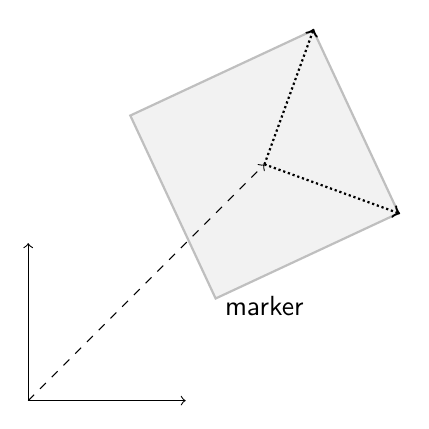
\begin{tikzpicture}[scale=1]

  \draw[->] (0, 0)--(0, 2);
  \draw[->] (0, 0)--(2, 0);

  \draw[draw=none,rotate around={20:(3, 3)}] (2, 2) rectangle (4, 4) node[fitting node, thick, rotate around={25:(0,0)}] (rect) {};

  \draw[dashed,->] (0, 0)--(3, 3);
  \draw[densely dotted, ->,thick] (3, 3)--(rect.north east);
  \draw[densely dotted, ->,thick] (3, 3)--(rect.south east);

  \node[] at (3, 1.2) {marker};
  
\end{tikzpicture}

\end{document}
